\documentclass[11pt,a4paper]{article}
\usepackage[pdftex]{color,graphicx}
\usepackage{tabularx}

% Uncomment the following two lines to check syntax only (no .dvi output produced, so it's faster!)
%\usepackage{syntonly}
%\syntaxonly

%\pagestyle{headings}

% Manual marging change
\addtolength{\topmargin}{-1cm}
\addtolength{\textheight}{2cm}

% Superscript and subscript commands
\newcommand{\superscript}[1]{\ensuremath{^{\textnormal{\scriptsize{#1}}}}}
\newcommand{\subscript}[1]{\ensuremath{_{\textnormal{\scriptsize{#1}}}}}

% Define the title
\title{CBMIA User's Guide}
\author{Matthieu Cattin}

\begin{document}

% Insert logos
\begin{figure}[t]
  
\includegraphics[height=3cm]{figures/cern_logo.pdf}
  \label{fig:cern_logo}
\end{figure}

% Generate the title
\maketitle

% Document abstract
\begin{abstract}
This document descibes the CBMIA board usage for firmware version 2.00 and older.
The CBMIA is a MIL1553 bus controller in PCI form-factor.

\end{abstract}


% Revision history
\newpage
\begin{tabularx}{1.0\textwidth}{| c | c | l | X |}
\hline
Revision & Date & Author &  Comments\\
\hline
0.1 & 19.06.2012 & Matthieu CATTIN & Initial revision\\
\hline
\end{tabularx}

% Insert a table of content
\newpage
\tableofcontents

% Start sections on a new page
\newpage

%===============================================================================
\section{Overview}

At CERN MIL1553 is used to control several types of equipments (e.g. power converters).
CERN implementation of MIL1553 is based on MIL-STD-1553-B, but is not fully compliant to it.
Nevertheless, the encoding, the frames structure and the low level protocol are compliant.

The MIL1553 bus uses a command/response protocol. It is based on Manchester encoded 16-bit words.
Each word starts with an additional 3-bit synchronisation pattern and ends with an odd parity bit \footnotemark.
\footnotetext{See MIL-STD-1553B specification for further details.}

In this document, a command/response couple is called a transaction.
There is two types of transactions; "BC to RT" and RT to BC".
In any case, the transaction is initiated by the BC.
Writing a command word to the TX\_REG register will start a transaction.
Then a response from a RT is expected.
The end of a transaction is detected either when a RT finished sending a frame or upon response timeout.
The response timeout $t$ in seconds is set in hardware to:
\[
t = \frac{2^{10}-1}{40e^6} = 25.575us
\]
Note that according the the MIL-STD-1553 specification, a RT must reply to a BC request within the time period of 4 to 12us.
A response time counter starts just after the end of the BC transmission. It will generate an error in case of timeout (no reply from RT).
If enabled in the IRQ\_EN register, an interrupt request is generated at the end of a transaction.

\begin{figure}[h]
  \centering
  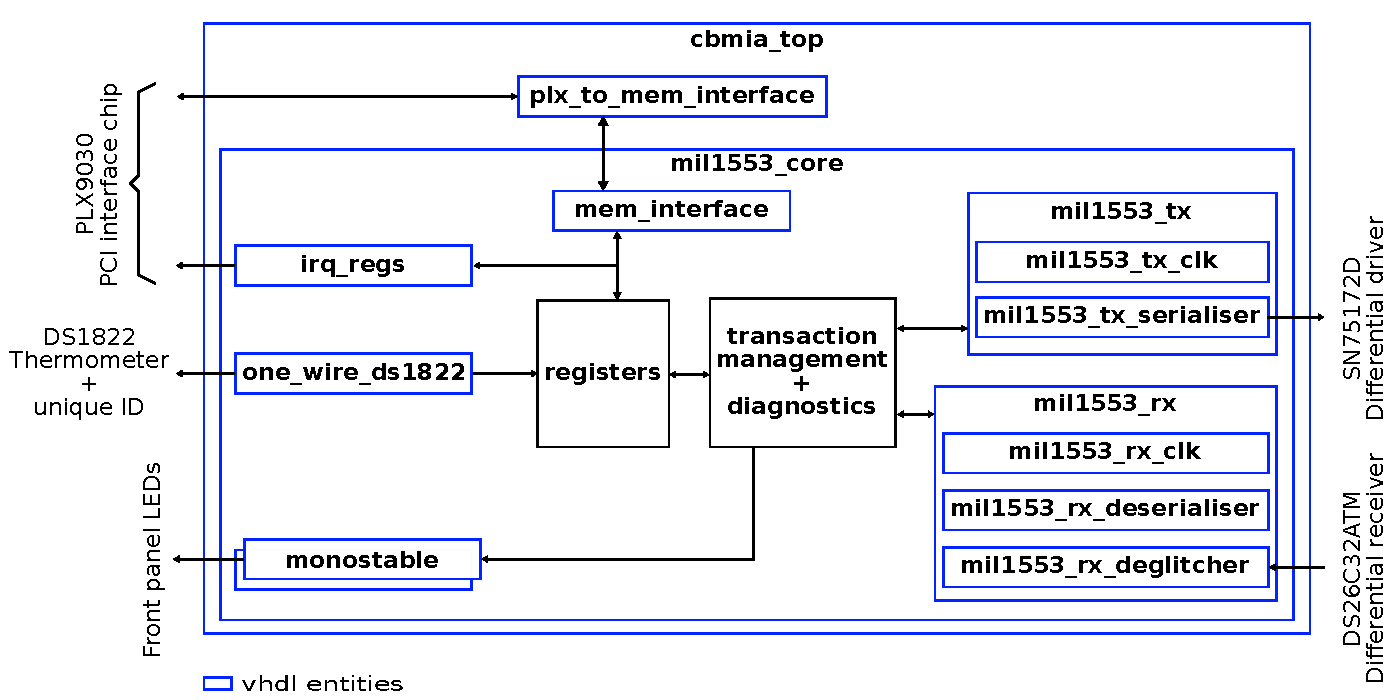
\includegraphics[width=0.99\textwidth]{figures/firmware_arch.pdf}
  \caption{CBMIA firmware architecure, only main entities and blocks are shown.}
  \label{fig:firmware_arch}
\end{figure}


%===============================================================================
\newpage
\section{Front panel LEDs}

\begin{table}[h!]
  \centering
  \begin{tabular}{ c l }
    \hline
    \textbf{LED nb} & \textbf{Description}\\
    \hline
    0 & Tx in progress \\
    1 & Parity error \\
    2 & Rx in progress \\
    3 & Manchester error \\
    4 & Response timeout \\
    5 & Number of word error \\
    6 & PCI bus access \\
    7 & Overwrite error \footnotemark \\
    \hline
  \end{tabular}
\end{table}

\footnotetext{Transmission request during a transaction will generate an error.}


%===============================================================================
\section{Glossary}

\begin{table}[h!]
  \centering
  \begin{tabularx}{\textwidth}{ l X }
    BC & : Bus Controller, this is a master on a MIL1553 bus. \\
    RT & : Remote Terminal, this is a slave on a MIL1553 bus. \\
    Transaction & : Command/response couple \\
    Frame & : One or more words send by either the BC or the RT. \\
    % & :  \\
  \end{tabularx}
\end{table}


%===============================================================================
\newpage
\section{Memory Map}
The register width is 32 bits. Addresses in the following table represents an offset from the first address of the PCI window.
The addresses are 32-bit words addresses.

\begin{table}[ht]
  \caption{\label{memory_map} CBMIA memory map.}
  \begin{tabularx}{\textwidth}{|l|l|l|X|}
    \hline
    \textbf{Address} & \textbf{Access} & \textbf{Description}\\
    \hline
    00         & CR  & Interrupt source \\
    01         & RW  & Interrupt enable mask \\
    02         & RO  & Temperature \\
    03         & RO  & Status register \\
    04         & RW  & Command register \\
    05         & RW  & Reserved \\
    06         & RO  & Unique ID (MSBs) \\
    07         & RO  & Unique ID (LSBs) \\
    08         & RW  & Transmit register \\
    09         & RO  & Receive register \\
    10 - 26  & RO    & Receive buffer \\
    27 - 42  & RW    & Transmit buffer \\
    43         & RO  & Transmitted frame counter \\
    44         & RO  & Reveived frame counter \\
    45         & RO  & Parity error counter \\
    46         & RO  & Manchester error counter \\
    47         & RO  & Number of word received error counter \\
    48         & RO  & Sent request during transaction error counter \\
    49         & RO  & Number of word transmitted, expected and received \\
    50         & RO  & RT response time \\
    51         & RO  & Reception error counter \\
    52         & RO  & Response timeout counter \\
    \hline
  \end{tabularx}
\end{table}

%===============================================================================
\newpage
\section{Registers detailed description}

%-------------------------------------------------------------------------------
\subsection{Interrupt source}

Name   : IRQ\_SRC \newline
Offset : 0 (0x0) \newline
Access : CR (Clear on read) \newline

\begin{table}[h!]
  \begin{tabularx}{\textwidth}{ l X }
    \hline
    \textbf{Fields} & \textbf{Description}\\
    \hline
    bit [0]     & End of transaction IRQ. \\
    bit [14:1]  & Unused. Ignore on read. \\
    bit [15]    & Reception error (FSM watchdog). \\
    bit [16]    & Response timeout (no reply from RT). \\
    bit [17]    & Number of received word differs from number of expected word (in the frame causing this IRQ). \\
    bit [18]    & Manchester error (in the frame causing this IRQ). \\
    bit [19]    & Parity error (in the frame causing this IRQ). \\
    bit [20]    & T/R flag, 0 = BC->RT transaction, 1 = RT->BC transaction. \\
    bit [26:21] & Word count. If T/R flag = 1, countains the number of word present in the receive buffer, including the status word. \\
    bit [31:27] & RT number, 0 = response timeout or truncated/corrupted frame. \\
    \hline
  \end{tabularx}
\end{table}

%-------------------------------------------------------------------------------
\subsection{Interrupt enable mask}

Name   : IRQ\_EN \newline
Offset : 1 (0x1) \newline
Access : WR (Read/write) \newline

\begin{table}[h!]
  \begin{tabularx}{\textwidth}{ l X }
    \hline
    \textbf{Fields} & \textbf{Description}\\
    \hline
    bit [0]     & 0 = Disables end of transaction IRQ, 1 = Enables end of transaction IRQ. \\
    bit [31:1]  & Unused. Ignore on read, write with 0. \\
    \hline
  \end{tabularx}
\end{table}

%-------------------------------------------------------------------------------
\subsection{Temperature}

Name   : TEMP \newline
Offset : 2 (0x2) \newline
Access : RO (Read only) \newline

Temperature of the board in degree Celsius.
The temperature value is refreshed every second.

\begin{table}[h!]
  \begin{tabularx}{\textwidth}{ l X }
    \hline
    \textbf{Fields} & \textbf{Description}\\
    \hline
    bit [3:0]   & Fractional part. \\
    bit [10:4]  & Integer part. \\
    bit [15:11] & Sign. \\
    bit [31:16] & Unused. Ignore on read. \\
    \hline
  \end{tabularx}
\end{table}

%-------------------------------------------------------------------------------
\subsection{Status register}

Name   : STAT \newline
Offset : 3 (0x3) \newline
Access : RO (Read only) \newline

\begin{table}[h!]
  \begin{tabularx}{\textwidth}{ l X }
    \hline
    \textbf{Fields} & \textbf{Description}\\
    \hline
    bit [15:0]  & BCD encoded HDL version (e.g. 0203 => v2.03). \\
    bit [30:16] & Unused. Ignore on read. \\
    bit [31]    & Transaction flag.
                  0 = MIL1553 bus is idle,
                  1 = Transaction in progress on MIL1553 bus. \\
    \hline
  \end{tabularx}
\end{table}

%-------------------------------------------------------------------------------
\subsection{Command register}

Name   : CMD \newline
Offset : 4 (0x4) \newline
Access : RW (Read/write) \newline

\begin{table}[h!]
  \begin{tabularx}{\textwidth}{ l X }
    \hline
    \textbf{Fields} & \textbf{Description}\\
    \hline
    bit [0]     & Software reset command. Write 1 to reset (automatically cleared). \\
    bit [15:1]  & Unused. Ignore on read, write with 0. \\
    bit [19:16] & Test point 0 mux (See mux correspondance table). \\
    bit [23:20] & Test point 1 mux (See mux correspondance table). \\
    bit [27:24] & Test point 2 mux (See mux correspondance table). \\
    bit [31:28] & Test point 3 mux (See mux correspondance table). \\
    \hline
  \end{tabularx}
\end{table}

%-------------------------------------------------------------------------------
\subsection{Reserved}

Name   : RFU \newline
Offset : 5 (0x5) \newline
Access : RO (Read only) \newline

\begin{table}[h!]
  \begin{tabularx}{\textwidth}{ l X }
    \hline
    \textbf{Fields} & \textbf{Description}\\
    \hline
    bit [31:0] & Unused. Ignore on read, write with 0. \\
    \hline
  \end{tabularx}
\end{table}

%-------------------------------------------------------------------------------
\subsection{Unique ID (MSBs)}

Name   : ID\_MSB \newline
Offset : 6 (0x6) \newline
Access : RO (Read only) \newline

\begin{table}[h!]
  \begin{tabularx}{\textwidth}{ l X }
    \hline
    \textbf{Fields} & \textbf{Description}\\
    \hline
    bit [31:0]  & Board's unique ID. MSBs of DS1822 64-bit unique ID. \\
    \hline
  \end{tabularx}
\end{table}

%-------------------------------------------------------------------------------
\subsection{Unique ID (LSBs)}

Name   : ID\_LSB \newline
Offset : 7 (0x7) \newline
Access : RO (Read only) \newline

\begin{table}[h!]
  \begin{tabularx}{\textwidth}{ l X }
    \hline
    \textbf{Fields} & \textbf{Description}\\
    \hline
    bit [31:0]  & Board's unique ID. LSBs of DS1822 64-bit unique ID. \\
    \hline
  \end{tabularx}
\end{table}

%-------------------------------------------------------------------------------
\subsection{Transmit register}

Name   : TX\_REG \newline
Offset : 8 (0x8) \newline
Access : RW (Read/write) \newline

\begin{table}[h!]
  \begin{tabularx}{\textwidth}{ l X }
    \hline
    \textbf{Fields} & \textbf{Description}\\
    \hline
    bit [4:0]   & Word count. \\
    bit [9:5]   & Sub-module address. \\
    bit [10]    & T/R. \\
    bit [15:11] & RT address. \\
    bit [31:16] & Unused. Ignore on read, write with 0. \\
    \hline
  \end{tabularx}
\end{table}

Bits [15:0] corresponds to the command word to be sent on the MIL1553 bus.
When this register is written, a transaction starts (if no other transaction are
in progress). If a transaction is already in progress, the request is ignored.

%-------------------------------------------------------------------------------
\subsection{Receive register}

Name   : RX\_REG \newline
Offset : 9 (0x9) \newline
Access : RO (Read only) \newline

\begin{table}[h!]
  \begin{tabularx}{\textwidth}{ l X }
    \hline
    \textbf{Fields} & \textbf{Description}\\
    \hline
    bit [15:0]  & RT status word of the last transaction. \\
    bit [31:16] & First received data word of the last transaction (if any, otherwise 0). \\
    \hline
  \end{tabularx}
\end{table}

%-------------------------------------------------------------------------------
\subsection{Receive buffer}

Name   : RX\_BUF \newline
Offset : 10-26 (0xA-0x1A) \newline
Access : RO (Read only) \newline

The receive buffer contains the last frame received from an RT.
Every buffer address contains two 16-bit words.
The first word is always the RT status, as defined in the MIL1553 protocol.
The receive buffer is reset to zero at the begining of a transaction.
In a transaction, it is mandatory for the RT to transmit at least its status.
Then in "RT to BC" transactions, the RT can send up to 32 words.
The number of word in the receive buffer, including the status word, is stored in the IRQ\_SRC register bit[26:21].

\begin{table}[h!]
  \centering
  \begin{tabular}{ c c c }
    \hline
    \textbf{Address} & \textbf{Upper 16-bit word} & \textbf{Lower 16-bit word}\\
    \hline
    10 & Data word 0 & RT status word \\
    11 & Data word 2 & Data word 1 \\
    ... & ... & ... \\
    25 & Data word 30 & Data word 29 \\
    26 & 0x0000 & Data word 31 \\
    \hline
  \end{tabular}
\end{table}

%-------------------------------------------------------------------------------
\subsection{Transmit buffer}

Name   : TX\_BUF \newline
Offset : 27-42 (0x1B-2A) \newline
Access : RW (Read/write) \newline

The transmit buffer contains the frame to be send to the RT.
In a "BC to RT" transaction, the BC can send up to 32 words to a RT.
The command word (first word in a frame) is taken from the TX\_REG register.

\begin{table}[h!]
  \centering
  \begin{tabular}{ c c c }
    \hline
    \textbf{Address} & \textbf{Upper 16-bit word} & \textbf{Lower 16-bit word}\\
    \hline
    27 & Data word 1 & Data word 0 \\
    28 & Data word 3 & Data word 2 \\
    ... & ... & ... \\
    41 & Data word 29 & Data word 28 \\
    42 & Data word 31 & Data word 30 \\
    \hline
  \end{tabular}
\end{table}

%-------------------------------------------------------------------------------
\subsection{Transmitted frame counter}

Name   : TX\_FRAME\_CNT \newline
Offset : 43 (0x2B) \newline
Access : RO (Read only) \newline

\begin{table}[h!]
  \begin{tabularx}{\textwidth}{ l X }
    \hline
    \textbf{Fields} & \textbf{Description}\\
    \hline
    bit [31:0]  & Transmitted frame counter. Cleared on reset. \\
    \hline
  \end{tabularx}
\end{table}

%-------------------------------------------------------------------------------
\subsection{Reveived frame counter}

Name   : RX\_FRAME\_CNT \newline
Offset : 44 (0x2C) \newline
Access : RO (Read only) \newline

\begin{table}[h!]
  \begin{tabularx}{\textwidth}{ l X }
    \hline
    \textbf{Fields} & \textbf{Description}\\
    \hline
    bit [31:0]  & Received frame counter. Cleared on reset. \\
    \hline
  \end{tabularx}
\end{table}

%-------------------------------------------------------------------------------
\subsection{Parity error counter}

Name   : PARITY\_ERR\_CNT \newline
Offset : 45 (0x2D) \newline
Access : RO (Read only) \newline

\begin{table}[h!]
  \begin{tabularx}{\textwidth}{ l X }
    \hline
    \textbf{Fields} & \textbf{Description}\\
    \hline
    bit [31:0]  & Parity error counter. Incermented on parity error in the received frame. Cleared on reset. \\
    \hline
  \end{tabularx}
\end{table}

%-------------------------------------------------------------------------------
\subsection{Manchester error counter}

Name   : MANCH\_ERR\_CNT \newline
Offset : 46 (0x2E) \newline
Access : RO (Read only) \newline

\begin{table}[h!]
  \begin{tabularx}{\textwidth}{ l X }
    \hline
    \textbf{Fields} & \textbf{Description}\\
    \hline
    bit [31:0]  & Manchester encoding error. Incermented on Manchester encoding error in the received frame. Cleared on reset. \\
    \hline
  \end{tabularx}
\end{table}

%-------------------------------------------------------------------------------
\subsection{Number of word received error counter}

Name   : NB\_WORD\_ERR\_CNT \newline
Offset : 47 (0x2F) \newline
Access : RO (Read only) \newline

\begin{table}[h!]
  \begin{tabularx}{\textwidth}{ l X }
    \hline
    \textbf{Fields} & \textbf{Description}\\
    \hline
    bit [31:0]  & Number of word error counter. Incermented when the number of received words is different from the expected number of words. Cleared on reset. \\
    \hline
  \end{tabularx}
\end{table}

%-------------------------------------------------------------------------------
\subsection{Sent request during transaction error counter}

Name   : TX\_ERR\_CNT \newline
Offset : 48 (0x30) \newline
Access : RO (Read only) \newline

\begin{table}[h!]
  \begin{tabularx}{\textwidth}{ l X }
    \hline
    \textbf{Fields} & \textbf{Description}\\
    \hline
    bit [31:0]  & Transmission error counter. Incremented when a transmission request (write to TX\_REG) arrives during a transaction. Cleared on reset. \\
    \hline
  \end{tabularx}
\end{table}

%-------------------------------------------------------------------------------
\subsection{Number of word transmitted, expected and received}

Name   : NB\_WORD \newline
Offset : 49 (0x31) \newline
Access : RO (Read only) \newline

\begin{table}[h!]
  \begin{tabularx}{\textwidth}{ l X }
    \hline
    \textbf{Fields} & \textbf{Description}\\
    \hline
    bit [5:0]   & Word count transmitted (for BC->RT and RT->BC). \\
    bit [11:6]  & Word count received (for RT->BC only). \\
    bit [17:12] & Expected number of word (for BC->RT and RT->BC). \\
    bit [25:18] & Unused. Ignore on read. \\
    bit [26]    & Reception error (FSM watchdog). \\
    bit [27]    & Response timeout (no reply from RT). \\
    bit [28]    & Number of received word differs from number of expected word (in the frame causing this IRQ). \\
    bit [29]    & Manchester error (in the frame causing this IRQ). \\
    bit [30]    & Parity error (in the frame causing this IRQ). \\
    bit [31]    & T/R flag, 0 = BC->RT transaction, 1 = RT->BC transaction. \\
    \hline
  \end{tabularx}
\end{table}

%-------------------------------------------------------------------------------
\subsection{RT response time}

Name   : RESP\_TIME \newline
Offset : 50 (0x32) \newline
Access : RO (Read only) \newline

\begin{table}[h!]
  \begin{tabularx}{\textwidth}{ l X }
    \hline
    \textbf{Fields} & \textbf{Description}\\
    \hline
    bit [9:0]   & Response timeout counter value. Can be used to measure the RT response time. \\
    bit [31:10] & Unused. Ignore on read. \\
    \hline
  \end{tabularx}
\end{table}

Response time $t$ in seconds is calculated as follow:

\[
t = \frac{1023 - counter\_value}{40e^6}
\]

If Response timeout counter value is 1023, it means that a the RT didn't reply and a timeout occured.

%-------------------------------------------------------------------------------
\subsection{Reception error counter}

Name   : RX\_ERROR\_CNT \newline
Offset : 51 (0x33) \newline
Access : RO (Read only) \newline

\begin{table}[h!]
  \begin{tabularx}{\textwidth}{ l X }
    \hline
    \textbf{Fields} & \textbf{Description}\\
    \hline
    bit [31:0]  & Reception error counter. Incremented if the bus is idle for more than 3.2us during a frame reception (-> FSM watchdog). Cleared on reset. \\
    \hline
  \end{tabularx}
\end{table}

%-------------------------------------------------------------------------------
\subsection{Response timeout counter}

Name   : RESP\_TIMEOUT\_CNT \newline
Offset : 52 (0x34) \newline
Access : RO (Read only) \newline

\begin{table}[h!]
  \begin{tabularx}{\textwidth}{ l X }
    \hline
    \textbf{Fields} & \textbf{Description}\\
    \hline
    bit [31:0]  & Response timeout counter. Incremented on RT response timeout. Cleared on reset. \\
    \hline
  \end{tabularx}
\end{table}


\end{document}
